Denne sektion er baseret på \citet{art:essence}.

Konfigurationstabellen, \cref{tab:konfigurationsTabel}, der er beskrevet i denne sektion er den første konfigurationstabel af systemet.
Grunden til dette er fordi metoden kun skal være en grundsten for videre arbejde.
Når man skal lave videre arbejde er det vigtigt at kigge på de findings der er beskrevet i en konfigurationstabel.
Denne del er dog ikke udfyldt på grund af der ikke er fundet nogle findings endnu, disse vil dog blive beskrevet senere i \cref{sec:findings}.
Denne konfigurationstabel har mange ligheder med den der er beskrevet i \citet{misc:faellesrapp}.
Grunden til dette er fordi det er samme målgruppe der udvikles til, endvidere udvikles der til PsyLog platformen der blev udviklet i \citet{misc:faellesrapp}.

\begin{figure}[]\centering
	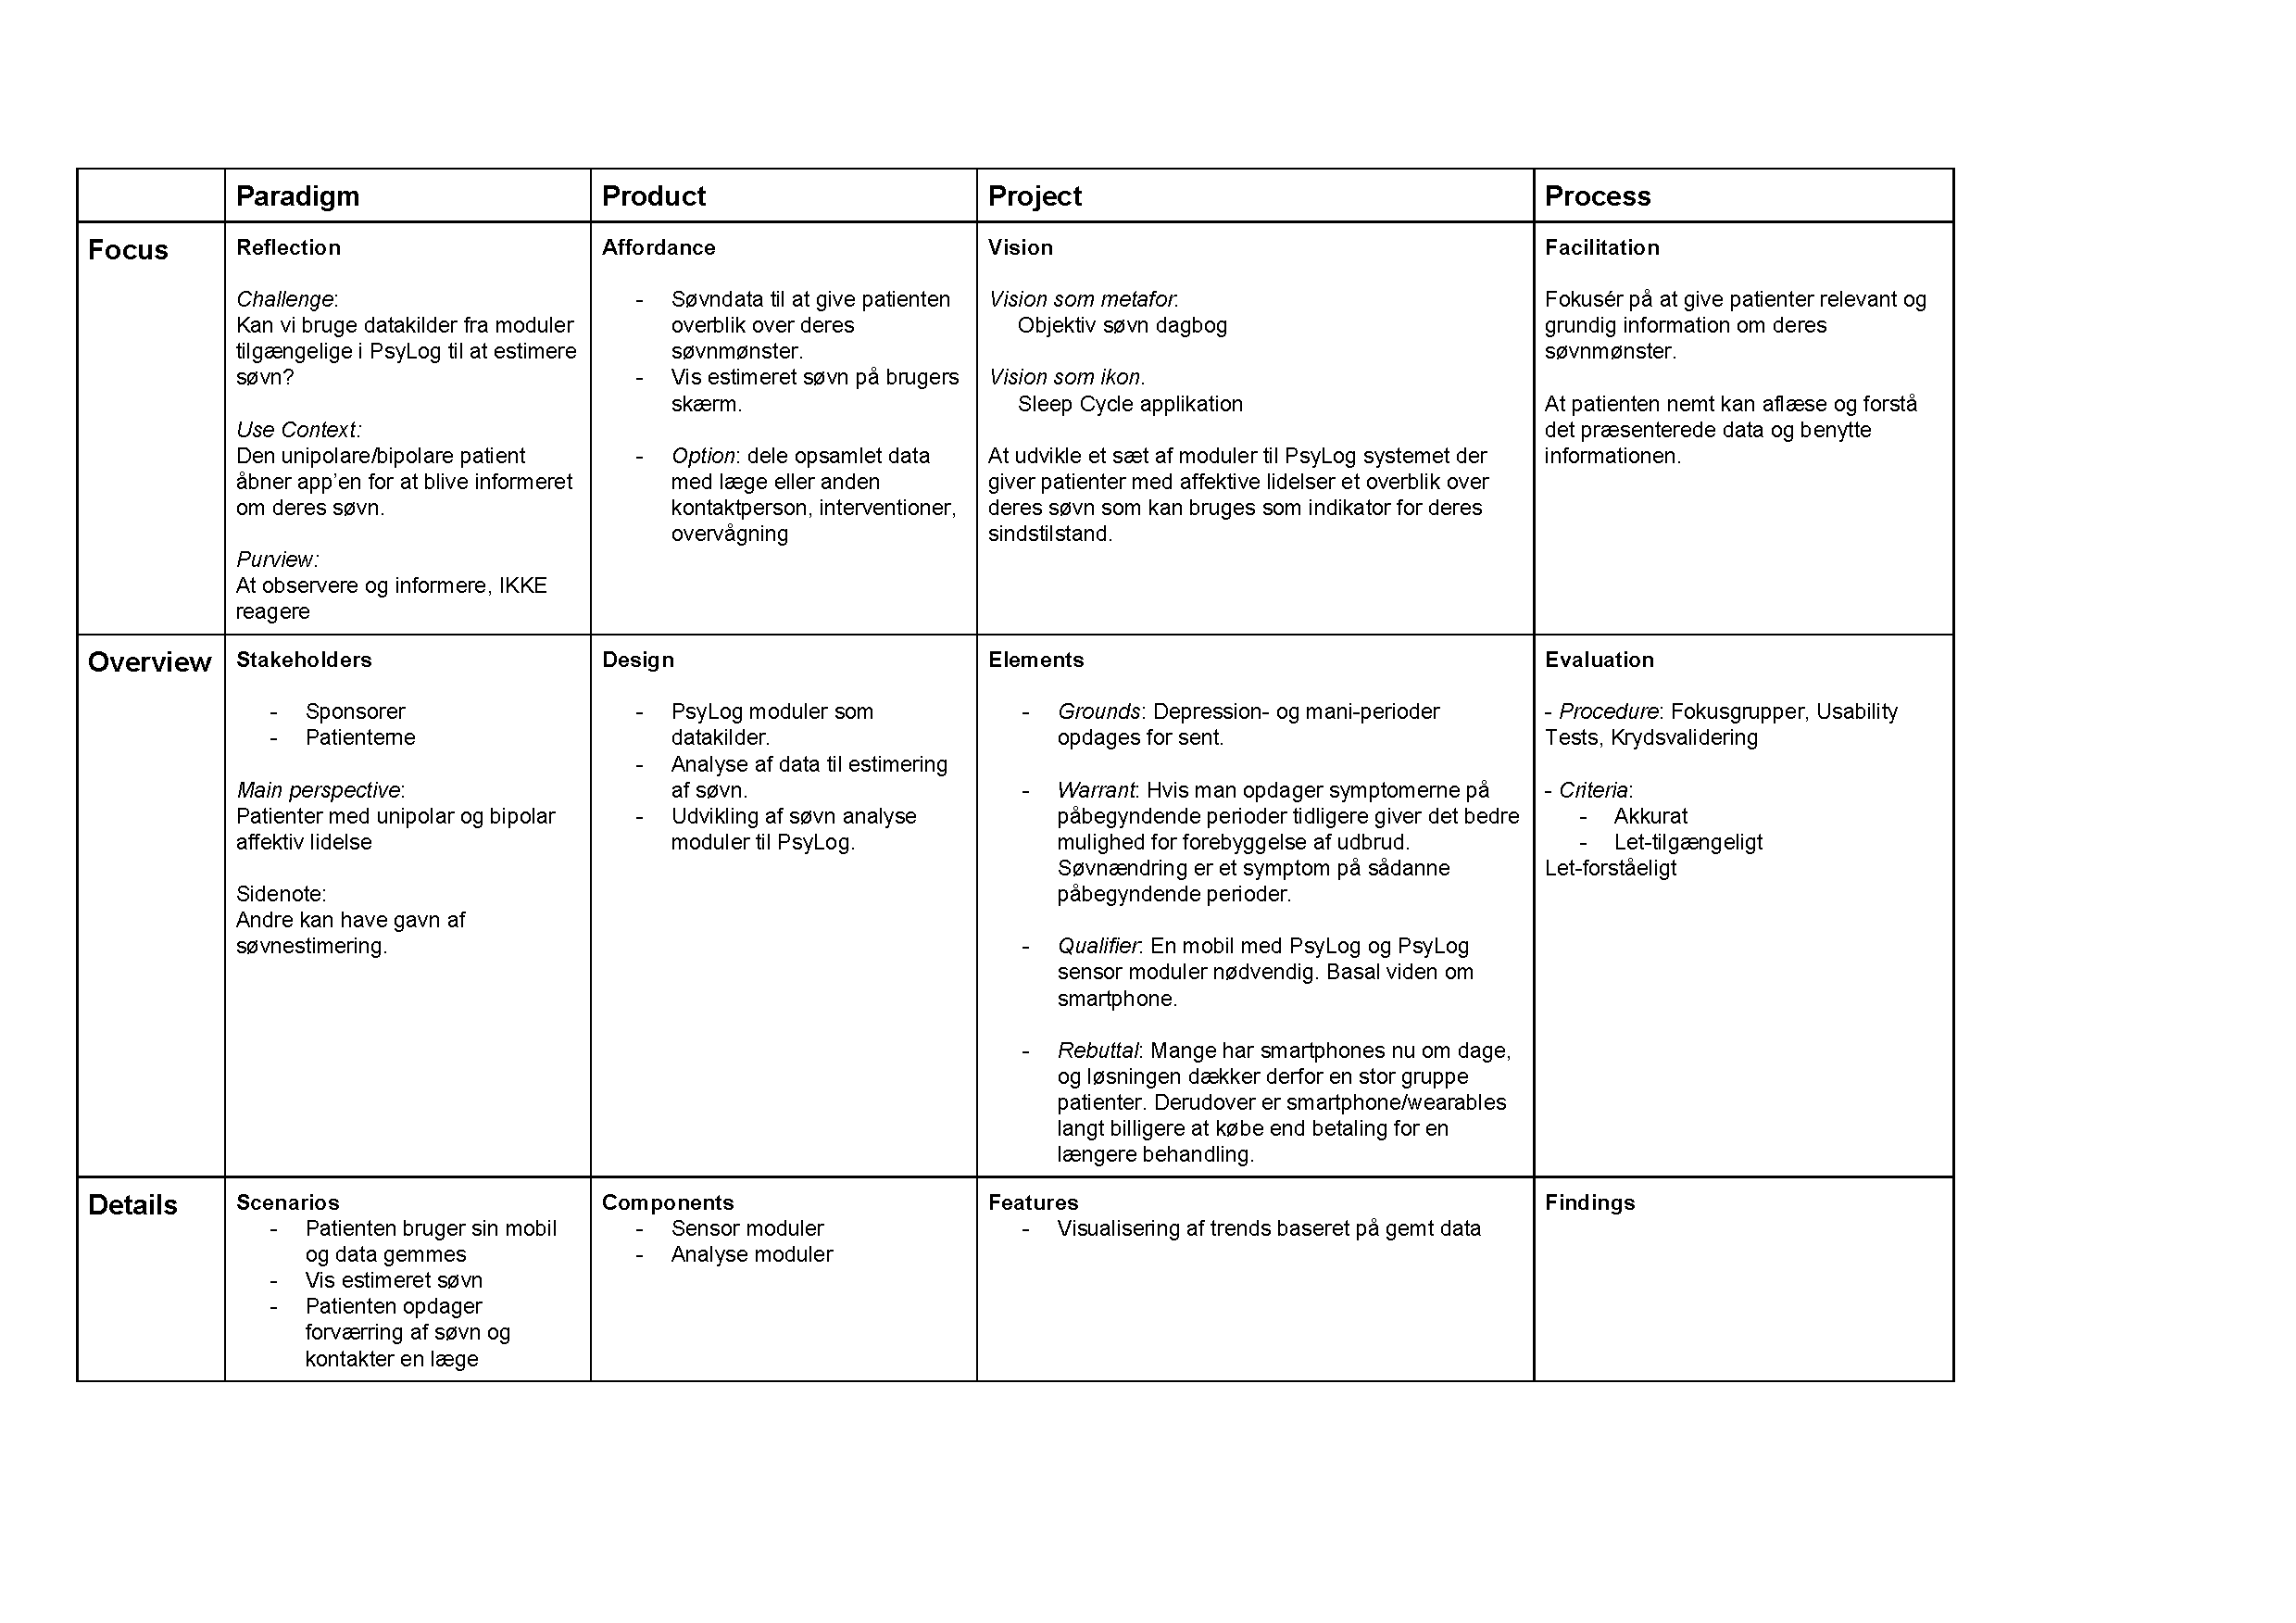
\includegraphics[scale = 0.65, angle =90,trim = 1cm 3cm 6cm 2cm, clip]{konfigurationstabel}
	\caption{Konfigurations tabellen for systemet.}
	\label{tab:konfigurationsTabel}
\end{figure}

En konfigurationstabel er lavet fordi det er vigtigt at alle udviklere ser på projektet på samme måde, så alle ved lige præcis hvad for et type projekt der arbejdes på, samt hvorfor lige præcis dette projekt udvikles.
Ydermere, giver konfigurationstabellen også et overblik over hvilket komponenter der kan bruges til at udvikle projektet, samt også hvilket begrænsninger der muligvis er i projektet.
Endvidere, beskriver konfigurationstabellen også en måde at evaluere projektet på, så alle ved præcis hvordan de skal evaluere vigtigheden af de forskellige opgaver.

Til at få udtrykt en vision for projektet som alle udviklere er indforstået med er der brugt både en metafor og et ikon.
Metaforen og ikon tjener hvert sit formål i forhold til visionen.

Metaforen som vision er knap så udtømmende, men er tiltænkt som en parallel man kan drage til en anden kontekst og går på koncept niveau mere end på faste specifikationer.
Metaforen for systemet er en objektiv søvn dagbog, dette er valgt fordi det er sensorer der samler data og vedhjælp af disse lave en historie omkring hvordan ens søvn har været.

Ikonet som vision skal forstås som et forbillede rent æstetisk, dvs. hvilket layout ens løsning skal følge.
Som ikon bruges \textit{Sleep Cycle} \citep{misc:sleepCycle}, hvilket er en alarm applikation som vækker en når man er i den lette søvn periode.
Den er set som et forbillede i den forstand at det er en ikke forstyrrende søvndetekterings applikation, hvilket for vores produkt ses som et helt centralt krav.